\documentclass[11pt,xcolor={dvipsnames},hyperref={pdftex,pdfpagemode=UseNone,hidelinks,pdfdisplaydoctitle=true},usepdftitle=false]{beamer}
\usepackage{presentation}

\hypersetup{pdftitle={Augmenting Model-Based Instantiation with Fast Enumeration}}
\newcommand\sym[1]{\mathsf{#1}}
\newcommand\ty[1]{\mathit{#1}}

\newcommand{\pt}{\phantom{0}}
\newcommand{\ptt}{\phantom{0}\phantom{0}}
\newcommand{\pttt}{\phantom{0}\phantom{0}\phantom{0}}
\newcommand{\ptttt}{\phantom{0}\phantom{0}\phantom{0}\phantom{0}}
\newcommand{\system}{\textsc{Goblin}}
\newcommand{\green}[1]{\textcolor{green!60!black}{#1}}
\newcommand{\red}[1]{\textcolor{red!70!black}{#1}}
\newcommand{\blue}[1]{\textcolor{blue!70!black}{#1}}
\newcommand{\teal}[1]{{\color{teal}{#1}}}
\newcommand{\highlight}{\makebox[0pt][l]{\color{lightgray}\rule[-2pt]{\linewidth}{9pt}}}
\definecolor{darkred}{rgb}{0.6,0.0,0.0} 
\definecolor{darkgreen}{RGB}{0,100,0}  
\definecolor{darkblue}{RGB}{0,0,175} 
\definecolor{lightgray}{gray}{0.85}

\newrobustcmd\B{\DeclareFontSeriesDefault[rm]{bf}{b}\bfseries} 
\usepackage{siunitx}
\usepackage{mdframed}
\usepackage{algorithmicx}
\usepackage{algpseudocode}
\usepackage[normalem]{ulem}
\usepackage{xcolor}
\usepackage{tikz}
\usepackage{listings}
\newcommand{\code}[1]{{\footnotesize\texttt{#1}}}
\setbeamercovered{invisible}  
% Define a custom dark green color
\definecolor{darkgreen}{rgb}{0.0, 0.5, 0.0}
\begin{document}
\lstdefinelanguage{Goblin}{
  sensitive=true,
  morekeywords=[1]{int_to_bv,length,mod,seq,len,set,singleton,union,member},
  morekeywords=[2]{BitVec,Int,Bool,List,Set,String},
  morekeywords=[3]{bvand,bvor,bvxor,bvnot,and,or,not,bvplus,bvugt,bvult,bvmul}
}

\lstdefinestyle{goblin}{
  language=Goblin,
  basicstyle=\ttfamily\scriptsize,
  numbers=left,
  numberstyle=\tiny\color{gray},
  xleftmargin=0em,
  stepnumber=1,
  frame=single,
  linewidth=.94\columnwidth,
  % framesep=4pt,
  showstringspaces=false,
  breaklines=true,
  tabsize=2,
  columns=fullflexible,
  commentstyle=\color{gray}\itshape,
  stringstyle=\color{red!70!black}, 
  keywordstyle=[1]\color{blue},
  keywordstyle=[2]\color{teal}\bfseries, 
  keywordstyle=[3]\color{purple}\bfseries,
  keepspaces,
  escapeinside={@}{@},
  % moredelim=[is][\color{anglemark}\bfseries]{<}{>},
literate=% 
    {0}{{{\color{darkred}0}}}1
    {0b}{{{\color{darkred}0b}}}1
    {1}{{{\color{darkred}1}}}1
    {2}{{{\color{darkred}2}}}1
    {3}{{{\color{darkred}3}}}1
    {4}{{{\color{darkred}4}}}1
    {5}{{{\color{darkred}5}}}1
    {6}{{{\color{darkred}6}}}1
    {7}{{{\color{darkred}7}}}1
    {8}{{{\color{darkred}8}}}1
    {9}{{{\color{darkred}9}}}1
    % {.}{{{\color{blue}.}}}1
    {-->}{{{$\leadsto$}}}1
    % {::}{{{\color{black}\bfseries ::}}}3%
    % {=}{{{\color{black}\bfseries =}}}3%
    % {<-}{{{\color{black}\bfseries <-}}}3%
    % {+}{{{\color{black}\bfseries +}}}3%
    % {|}{{{\color{black}\bfseries |}}}3%
    % {;}{{{\color{black}\bfseries ;}}}3%
    % {\{}{{{\color{black}\bfseries \{}}}3%
    % {\}}{{{\color{black}\bfseries \}}}}3%
    % {<}{{{\color{green}\bfseries <}}}3%
}


% \setstretch{1.25}
\setbeamerfont{title}{size=\Large}
\title{Parse this! \\ Summoning Context-Sensitive Inputs with \system{}}
%\subtitle{Extending SMT solving}

\information
%  
% []  
%
{\underline{Rob Lorch} \quad Muhammad Daniyal Pirwani Dar \newline \quad Cesare Tinelli \quad Omar Chowdhury
\newline \newline   
The University of Iowa
\newline    
Stony Brook University
}
%
%{TACAS 2025 \\2025-05-05, Hamilton, Canada}

\frame{\titlepage}

\begin{frame} 
    \frametitle{Problem Introduction} %\pause
    \begin{itemize}
        \item Some software systems have highly \green{complex input formats} (e.g. compilers, file renderers, network protocol stacks) \pause
        \item Complex input formats are difficult for testing, especially \green{automated testing} \pause
        \item We will discuss techniques for \green{automated input generation} of software with complex input formats \pause
        \item Given an input specification, how to generate inputs?
    \end{itemize}
    % What problem are we addressing?
    % Like paper introduction
    % Software sometimes has highly complex input formats, which are difficult for automated testing, 
    %   especially if blackbox
    % In general, we are interest in the problem of automated testing of software with highly complex
    %   input spec
    % More concretely, we focus on the problem of **input generation**
    %   - we have a spec and we want to generate inputs
\end{frame}

\begin{frame} 
    \frametitle{Existing Approaches} 
    \begin{itemize}
        \item Use \green{context-free grammars} (CFGs) to capture input structure \pause
        \begin{itemize}
            \item HTTP requests, DNS packets, LangFuzz\pause
            \item Can only handle context-free aspects of the spec\pause
            \item Consider packet format with fields 
            \blue{$f_1$} and \blue{$f_2$} s.t. \blue{$f_1 = |f_2|$}\pause
        \end{itemize}
        \item Tools tailor-made for \green{system under test} (SUT)\pause
        \begin{itemize}
            \item CSmith\pause
            \item Lacks generality!\pause
        \end{itemize}
        \item \green{Coverage-guided mutation}\pause
        \begin{itemize}
            \item How to generate an initial corpus?\pause
            \item What if no access to coverage information?\pause
            \item Mutations still blind to specification constraints
        \end{itemize}
    \end{itemize}
    % Conceptually different approaches
    % Context-free grammar based fuzzing (examples)
    % General-purpose code (a la CSmith, examples)
    % Coverage-guided mutation
        % - how to generate an initial corpus? Back to square 1
        % - what if you don't have access to coverage information?
        % - even so, mutations are blind to the input constraints, performance can be poor
    % Give negatives of all
\end{frame}

\begin{frame} 
    \frametitle{Wishlist} 
    \begin{enumerate}
        \item Generality of CFG-based approaches\pause
        \item Expressiveness of tailor-made fuzzers\pause
    \end{enumerate}
    \center{
    \textbf{Refine CFG-based approaches to be more expressive,} \newline 
    \textbf{while maintaining their generality}}
    % We want the generality of CFG-based approaches
    % We want the expressiveness of tailormade solutions
    % First basic idea: Refine CFG-based approaches to be more expressive, while maintaining their generality
\end{frame}

\begin{frame}[fragile]
    \frametitle{Context-free input generation} 
  First, a CFG-based input generation example: XML! \\[4pt]\pause
\begin{lstlisting}[style=goblin]
<xml-tree> ::= <openclose-tag> | 
               <open-tag> <inner-tree> <close-tag>
               
<inner-tree> ::= <TEXT> | <xml-tree> 
               | <inner-tree> <inner-tree> 
                     
<open-tag>  ::= `<'  <id> `>' | `<' <id> ` ' <attribute> `>'
<close-tag> ::= `</' <id> `>'

<openclose-tag> := `<' <id> `/>' 
                 | `<' <id> ` ' <attribute> `/>'

<attribute> ::= <id> `="' <TEXT > `"' 
              | <attribute> ` ' <attribute> 
                    
<id> ::= <ID-START-CHAR> <ID-CHAR>* 
\end{lstlisting}
\end{frame}

\begin{frame}[fragile]
    \frametitle{Context-free input generation} 
Termination? (Mostly) well-formed inputs?
\begin{lstlisting}[style=goblin]
<xml-tree> ::= <openclose-tag> | 
               <open-tag> <inner-tree> <close-tag>
               
<inner-tree> ::= <TEXT> | <xml-tree> 
               | <inner-tree> <inner-tree> 
                     
<open-tag>  ::= `<'  <id> `>' | `<' <id> ` ' <attribute> `>'
<close-tag> ::= `</' <id> `>'

<openclose-tag> := `<' <id> `/>' 
                 | `<' <id> ` ' <attribute> `/>'

<attribute> ::= <id> `="' <TEXT > `"' 
              | <attribute> ` ' <attribute> 
                    
<id> ::= <ID-START-CHAR> <ID-CHAR>* 
\end{lstlisting}
\end{frame}

\begin{frame}[fragile]
    \frametitle{Introducing \system{}} 
    \begin{itemize}
        \item Presenting \system{} \pause
        \begin{itemize}
        \item A \green{context-sensitive input generation tool}, supported by \pause
        \item A new \green{DSL} with a formal semantics \pause
        \item A new \green{search algorithm} to address the underlying problem \pause
        \end{itemize}
        \item Given a context-sensitive grammar \blue{$G$}, find \blue{$x$} such that \blue{$x \in \mathcal{L}(G)$} \pause
        \item What is a context-sensitive grammar? 
\begin{lstlisting}[style=goblin]
<xml-tree> ::= <openclose-tag> | 
               <open-tag> <inner-tree> <close-tag>
             @\blue{\{ <open-tag>.<id> = <close-tag>.<id> \}}@
... 
\end{lstlisting}
    \end{itemize}
    % Context-sensitive input generator
    % Specific example (eg XML) 
    %   - input is grammar + constraints, output is XML input
    % Generalization (CFG, constraints, Goblin, serializer, parser)
\end{frame}



\begin{frame}
    \frametitle{Input generation vs fuzzing} 
    \system{} is an \green{input generator}, but not a (complete) \green{fuzzer} \\[8pt]\pause
        \resizebox{\linewidth}{!}{
        {\scriptsize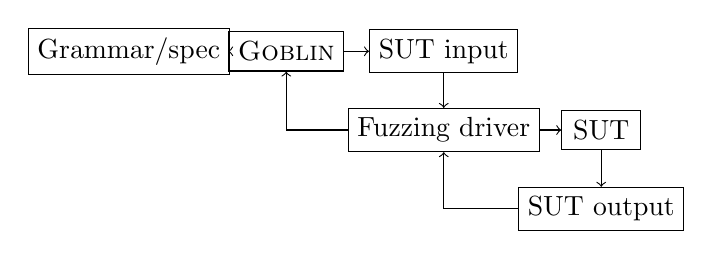
\begin{tikzpicture}[
            box/.style={draw, rectangle, minimum width=1cm, minimum height=.5cm, align=center}
            ]
 
            % Nodes with manual coordinates
            \node[box] (inp) at (0,2) {Grammar/spec};
            \node[box] (sys) at (2,2) {\system{}};
            \node[box] (sutinp) at (4,2) {SUT input};
            \node[box] (dr) at (4,1) {Fuzzing driver};
            \node[box] (sut) at (6,1) {SUT};
            \node[box] (sutout) at (6,0) {SUT output};

            % Arrows
            \draw[->] (inp.east) -- (sys.west);
            \draw[->] (sys.east) -- (sutinp.west);
            \draw[->] (sutinp.south) -- (dr.north);
            \draw[->] (dr.east) -- (sut.west);
            \draw[->] (dr.west) -| (sys.south);
            \draw[->] (sut.south) -- (sutout.north);
            \draw[->] (sutout.west) -| (dr.south);
        \end{tikzpicture}}}
\end{frame}

\begin{frame}
    \frametitle{Input generation vs fuzzing} 
    \system{} is an \green{input generator}, but not a (complete) \green{fuzzer} \\[8pt]
        \resizebox{\linewidth}{!}{
        {\scriptsize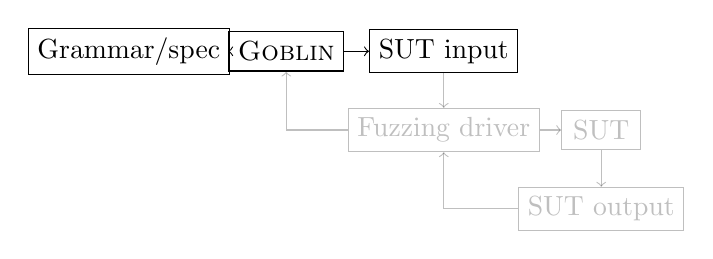
\begin{tikzpicture}[
            box/.style={draw, rectangle, minimum width=1cm, minimum height=.5cm, align=center}
            ]
 
            % Nodes with manual coordinates
            \node[box] (inp) at (0,2) {Grammar/spec};
            \node[box] (sys) at (2,2) {\system{}};
            \node[box] (sutinp) at (4,2) {SUT input};
            \begin{scope}[opacity=0.25] 
            \node[box] (dr) at (4,1) {Fuzzing driver};
            \node[box] (sut) at (6,1) {SUT};
            \node[box] (sutout) at (6,0) {SUT output};
            \end{scope}

            % Arrows
            \draw[->] (inp.east) -- (sys.west);
            \draw[->] (sys.east) -- (sutinp.west);
            \begin{scope}[opacity=0.25] 
            \draw[->] (sutinp.south) -- (dr.north);
            \draw[->] (dr.east) -- (sut.west);
            \draw[->] (dr.west) -| (sys.south);
            \draw[->] (sut.south) -- (sutout.north);
            \draw[->] (sutout.west) -| (dr.south);
            \end{scope}
        \end{tikzpicture}}}

        % \item Example: SAECRED (overlay workflow with SAECRED components)
        From now on we only discuss \green{input generation}
\end{frame}

\begin{frame}[fragile]
    \frametitle{\system{} by example: Language features}
\system{} grammars have \green{production rules} as in CFGs\\[4pt]
\begin{lstlisting}[style=goblin]
@\highlight@@\color{darkred}<PACKET>@ ::= @\color{teal}<TYPE>@ @\color{teal}<AUX>@ @\color{darkred}<PAYLOAD>@;



@\highlight@@\color{darkred}<PAYLOAD>@ ::= @\color{teal}<F1>@ @\color{teal}<F2>@ @\color{darkred}<BYTES>@; 

@\highlight@@\color{darkred}<BYTES>@ ::= @\color{teal}<BYTE>@ @\color{darkred}<BYTES>@ | @\color{teal}<BYTE>@ | @\color{teal}<OPT>@;



 @\;@
\end{lstlisting}
\end{frame}

\begin{frame}[fragile]
    \frametitle{\system{} by example: Language features}
Use \green{symbolic terminals} (in \teal {teal}) with \green{type annotations} rather than 
concrete terminals. Capture \green{abstract syntax}, not \green{concrete syntax}\\[4pt]
\begin{lstlisting}[style=goblin]
@\color{darkred}<PACKET>@ ::= @\color{teal}<TYPE>@ @\color{teal}<AUX>@ @\color{darkred}<PAYLOAD>@;



@\color{darkred}<PAYLOAD>@ ::= @\color{teal}<F1>@ @\color{teal}<F2>@ @\color{darkred}<BYTES>@; 

@\color{darkred}<BYTES>@ ::= @\color{teal}<BYTE>@ @\color{darkred}<BYTES>@ | @\color{teal}<BYTE>@ | @\color{teal}<OPT>@;
@\highlight@@\color{teal}<TYPE>@ :: BitVec(8);
@\highlight@@\color{teal}<BYTE>@ :: BitVec(8); 
@\highlight@@\color{teal}<AUX>@ :: BitVec(8); 
@\highlight@@\color{teal}<F1>@ :: BitVec(8); @\color{teal}<F2>@ :: BitVec(8); @\color{teal}<OPT>@ :: BitVec(4); 
\end{lstlisting}
\end{frame}

\begin{frame}[fragile]
    \frametitle{\system{} by example: Language features}
Constrain symbolic terminals with \green{refinement types}\\[4pt]
\begin{lstlisting}[style=goblin]
@\color{darkred}<PACKET>@ ::= @\color{teal}<TYPE>@ @\color{teal}<AUX>@ @\color{darkred}<PAYLOAD>@;



@\color{darkred}<PAYLOAD>@ ::= @\color{teal}<F1>@ @\color{teal}<F2>@ @\color{darkred}<BYTES>@; 

@\color{darkred}<BYTES>@ ::= @\color{teal}<BYTE>@ @\color{darkred}<BYTES>@ | @\color{teal}<BYTE>@ | @\color{teal}<OPT>@;
@\highlight@@\color{teal}<TYPE>@ :: BitVec(8) { @\color{teal}<TYPE>@ = 0x01 or @\color{teal}<TYPE>@ = 0x02; };   
@\highlight@@\color{teal}<BYTE>@ :: BitVec(8) { @\color{teal}<BYTE>@ bvult 0x88;}; 
@\color{teal}<AUX>@ :: BitVec(8); 
@\color{teal}<F1>@ :: BitVec(8); @\color{teal}<F2>@ :: BitVec(8); @\color{teal}<OPT>@ :: BitVec(4); 
\end{lstlisting}
\end{frame}

\begin{frame}[fragile]
    \frametitle{\system{} by example: Language features}
Attach \green{semantic constraits} to production rules

Support types/functions/predicates with \green{SMT-LIB} analogues\\[4pt]
\begin{lstlisting}[style=goblin]
@\color{darkred}<PACKET>@ ::= @\color{teal}<TYPE>@ @\color{teal}<AUX>@ @\color{darkred}<PAYLOAD>@
@\highlight@  { @\color{teal}<AUX>@ <- @\color{darkred}<PAYLOAD>@.@\color{teal}<F1>@ bvmul @\color{darkred}<PAYLOAD>@.@\color{teal}<F2>@;
@\highlight@    @\color{teal}<TYPE>@ = 0x01 => (@\color{darkred}<PAYLOAD>@.@\color{darkred}<BYTES>@.@\color{teal}<BYTE>@ bvugt 0x20 
@\highlight@                and @\color{darkred}<PAYLOAD>@.@\color{darkred}<BYTES>@.@\color{teal}<BYTE>@ bvult 0x7E); };
@\color{darkred}<PAYLOAD>@ ::= @\color{teal}<F1>@ @\color{teal}<F2>@ @\color{darkred}<BYTES>@ 
@\highlight@ { @\color{darkred}<BYTES>@.@\color{teal}<OPT>@ bvugt 0x0; };
@\color{darkred}<BYTES>@ ::= @\color{teal}<BYTE>@ @\color{darkred}<BYTES>@ | @\color{teal}<BYTE>@ | @\color{teal}<OPT>@;
@\color{teal}<TYPE>@ :: BitVec(8) { @\color{teal}<TYPE>@ = 0x01 or @\color{teal}<TYPE>@ = 0x02; };   
@\color{teal}<BYTE>@ :: BitVec(8) { @\color{teal}<BYTE>@ bvult 0x88;}; 
@\color{teal}<AUX>@ :: BitVec(8); 
@\color{teal}<F1>@ :: BitVec(8); @\color{teal}<F2>@ :: BitVec(8); @\color{teal}<OPT>@ :: BitVec(4); 
\end{lstlisting}
\end{frame}

\begin{frame}[fragile]
    \frametitle{\system{} by example: Language features}
Reference child nonterminals with \green{dot notation}\\[4pt]
\begin{lstlisting}[style=goblin]
@\color{darkred}<PACKET>@ ::= @\color{teal}<TYPE>@ @\color{teal}<AUX>@ @\color{darkred}<PAYLOAD>@
@\highlight@  { @\color{teal}<AUX>@ <- @\color{darkred}<PAYLOAD>@.@\color{teal}<F1>@ bvmul @\color{darkred}<PAYLOAD>@.@\color{teal}<F2>@;
@\highlight@    @\color{teal}<TYPE>@ = 0x01 => (@\color{darkred}<PAYLOAD>@.@\color{darkred}<BYTES>@.@\color{teal}<BYTE>@ bvugt 0x20 
@\highlight@                and @\color{darkred}<PAYLOAD>@.@\color{darkred}<BYTES>@.@\color{teal}<BYTE>@ bvult 0x7E); };
@\color{darkred}<PAYLOAD>@ ::= @\color{teal}<F1>@ @\color{teal}<F2>@ @\color{darkred}<BYTES>@ 
@\highlight@ { @\color{darkred}<BYTES>@.@\color{teal}<OPT>@ bvugt 0x0; };
@\color{darkred}<BYTES>@ ::= @\color{teal}<BYTE>@ @\color{darkred}<BYTES>@ | @\color{teal}<BYTE>@ | @\color{teal}<OPT>@;
@\color{teal}<TYPE>@ :: BitVec(8) { @\color{teal}<TYPE>@ = 0x01 or @\color{teal}<TYPE>@ = 0x02; };   
@\color{teal}<BYTE>@ :: BitVec(8) { @\color{teal}<BYTE>@ bvult 0x88;}; 
@\color{teal}<AUX>@ :: BitVec(8); 
@\color{teal}<F1>@ :: BitVec(8); @\color{teal}<F2>@ :: BitVec(8); @\color{teal}<OPT>@ :: BitVec(4); 
\end{lstlisting}
\end{frame}

\begin{frame}[fragile]
    \frametitle{\system{} by example: Language features}
Dot notation is \green{partial} and \green{implicitly universally quantified}\\[4pt]
\begin{lstlisting}[style=goblin]
@\color{darkred}<PACKET>@ ::= @\color{teal}<TYPE>@ @\color{teal}<AUX>@ @\color{darkred}<PAYLOAD>@
  { @\color{teal}<AUX>@ <- @\color{darkred}<PAYLOAD>@.@\color{teal}<F1>@ bvmul @\color{darkred}<PAYLOAD>@.@\color{teal}<F2>@;
    @\color{teal}<TYPE>@ = 0x01 => (@\color{darkred}<PAYLOAD>@.@\color{darkred}<BYTES>@.@\color{teal}<BYTE>@ bvugt 0x20 
                and @\color{darkred}<PAYLOAD>@.@\color{darkred}<BYTES>@.@\color{teal}<BYTE>@ bvult 0x7E); };
@\color{darkred}<PAYLOAD>@ ::= @\color{teal}<F1>@ @\color{teal}<F2>@ @\color{darkred}<BYTES>@ 
@\highlight@ { @\color{darkred}<BYTES>@.@\color{teal}<OPT>@ bvugt 0x0; };
@\color{darkred}<BYTES>@ ::= @\color{teal}<BYTE>@ @\color{darkred}<BYTES>@ | @\color{teal}<BYTE>@ | @\color{teal}<OPT>@;
@\color{teal}<TYPE>@ :: BitVec(8) { @\color{teal}<TYPE>@ = 0x01 or @\color{teal}<TYPE>@ = 0x02; };   
@\color{teal}<BYTE>@ :: BitVec(8) { @\color{teal}<BYTE>@ bvult 0x88;}; 
@\color{teal}<AUX>@ :: BitVec(8); 
@\color{teal}<F1>@ :: BitVec(8); @\color{teal}<F2>@ :: BitVec(8); @\color{teal}<OPT>@ :: BitVec(4); 
\end{lstlisting}
\end{frame}

\begin{frame}[fragile]
    \frametitle{\system{} by example: Language features}
Many constraints are not amenable to \green{automated constraint solving} 
with an \green{SMT engine}\\[4pt]
\begin{lstlisting}[style=goblin]
@\color{darkred}<PACKET>@ ::= @\color{teal}<TYPE>@ @\color{teal}<AUX>@ @\color{darkred}<PAYLOAD>@
@\highlight@  { @\color{teal}<AUX>@ <- @\color{darkred}<PAYLOAD>@.@\color{teal}<F1>@ bvmul @\color{darkred}<PAYLOAD>@.@\color{teal}<F2>@;
...
@\color{darkred}<PAYLOAD>@ ::= @\color{teal}<F1>@ @\color{teal}<F2>@ @\color{darkred}<BYTES>@ 
...
\end{lstlisting}\pause
\green{Derived fields} with \texttt{<-} denote nonterminals that are directly computable, enforced syntactically \pause

Cryptographic hashes, checksums, or \green{any computable function}
\end{frame}

\usetikzlibrary{trees,arrows.meta,matrix,positioning,calc,fit,shapes.geometric}
\tikzset{
  >=Latex,                             % nice arrowheads
  proc/.style = {draw, rounded corners, thick, fill=white, inner sep=6pt, minimum width=2cm, align=center},
  flow/.style = {->, thick},           % arrow style
  lab/.style  = {font=\small, midway, above} % label style
  io/.style   = {proc, trapezium, trapezium stretches=true,
                 trapezium left angle=70, trapezium right angle=110,
                 fill=gray!15, very thick}
} 
\begin{frame} 
    \frametitle{Semantics: Abstract syntax trees}
% \begin{itemize}
    \system{} generates \green{abstract syntax trees}, not strings\pause
%     \item AST view with SMT-LIB types enables constraint solving over SMT theories 
%     (prior work only natively supports string constraints)
% \end{itemize}


\newcommand{\dttree}{%
    \begin{tikzpicture}[
      scale=0.7, transform shape,
      level distance=14mm,
      level 1/.style={sibling distance=45mm},
      level 2/.style={sibling distance=25mm},
      leaf/.style={draw, ellipse, inner sep=2pt}
    ]
      \node {1: $\langle$Packet$\rangle[0]$} [-to]
        child { node {2: $\langle$Type$\rangle[0]$}
          child { node[leaf] {5: $0x01$} }}
        child { node {3: $\langle$Aux$\rangle[0]$}
          child { node[leaf] {6: $0x06$} } }
        child { node {4: $\langle$Payload$\rangle[0]$} 
          child { node {7: $\langle$F1$\rangle[0]$} child { node[leaf] {10: $0x02$} } }
          child { node {8: $\langle$F2$\rangle[0]$} child { node[leaf] {11: $0x03$} } }
          child { node {9: $\langle$Bytes$\rangle[0]$} child { node {12: $\langle$Byte$\rangle[1]$} child { node[leaf] {13: $0x21$} } } } };
    \end{tikzpicture}%
  }
  {\center \dttree} \pause 

  \green{Not} a string {\scriptsize \texttt{0b000000010000011000000010001100100001}}
% Grammar producing a string vs grammar producing an ADT term
% In the ADT view, we model derivations in progress as derivation trees
% Informally, the semantics of a Goblin input is the set of closed derivation trees 
%   that (i)  respect the context-free grammar rules and 
%        (ii) satisfy the constraints at every production rule application
\end{frame}

\begin{frame}
    \frametitle{Semantics: Abstract syntax trees}
    \begin{itemize}
        \item Without the AST view, prior work natively \green{only supports string constraints} \pause
        \item AST semantics position \system{} as a generator of constrained \green{algebraic datatype} (ADT) terms\pause
    \end{itemize}
    \center {\textbf{The ADT view allows \system{} to natively support constraints over arbitrary SMT theories}}
\end{frame}

\begin{frame} 
    \frametitle{Semantics}
    \blue{$\mathcal{L}_{\mathsf{AST}}(G) = \{ t \mid $}
\begin{enumerate}
    \item \blue{$t$} is rooted at the start symbol\pause
    \item Each \blue{$v \in V(t)$} is either \pause
    \begin{enumerate}
        \item A non-leaf with children representing a production rule application in \blue{$G$},\pause
        \item A non-leaf representing a type annotation in \blue{$G$}, or\pause
        \item A well-typed leaf\pause
    \end{enumerate}
    \item \blue{$t$} satisfies the constraints at every production rule application
\end{enumerate}
    \blue{$\}$}
\end{frame}

\begin{frame} [fragile]
    \frametitle{Semantics: Constraint Satisfaction}
 \begin{lstlisting}[style=goblin]
@\color{darkred}<PACKET>@ ::= @\color{teal}<TYPE>@ @\color{teal}<AUX>@ @\color{darkred}<PAYLOAD>@
@\highlight@  { @\color{teal}<AUX>@ <- @\color{darkred}<PAYLOAD>@.@\color{teal}<F1>@ bvmul @\color{darkred}<PAYLOAD>@.@\color{teal}<F2>@;
...
@\color{darkred}<PAYLOAD>@ ::= @\color{teal}<F1>@ @\color{teal}<F2>@ @\color{darkred}<BYTES>@ 
...
\end{lstlisting}

\newcommand{\dttree}{%
    \begin{tikzpicture}[
      scale=0.7, transform shape,
      level distance=14mm,
      level 1/.style={sibling distance=45mm},
      level 2/.style={sibling distance=25mm},
      leaf/.style={draw, ellipse, inner sep=2pt}
    ]
      \node {1: $\langle$Packet$\rangle[0]$} [-to]
        child[opacity=.5] { node {2: $\langle$Type$\rangle[0]$}
          child { node[leaf] {5: $0x01$} }}
        child { node {3: $\langle$Aux$\rangle[0]$}
          child { node[leaf] {6: $0x06$} } }
        child { node {4: $\langle$Payload$\rangle[0]$} 
          child { node {7: $\langle$F1$\rangle[0]$} child { node[leaf] {10: $0x02$} } }
          child { node {8: $\langle$F2$\rangle[0]$} child { node[leaf] {11: $0x03$} } }
          child[opacity=.5] { node {9: $\langle$Bytes$\rangle[0]$} child { node {12: $\langle$Byte$\rangle[1]$} child { node[leaf] {13: $0x21$} } } } };
    \end{tikzpicture}%
  }
  {\center \dttree}
\end{frame}

\begin{frame} [fragile]
    \frametitle{Semantics: Constraint Satisfaction}
 \begin{lstlisting}[style=goblin]
...
@\color{teal}<BYTE>@ :: BitVec(8) { @\color{teal}<BYTE>@ bvult 0x88;}; 
...
\end{lstlisting}

\newcommand{\dttree}{%
    \begin{tikzpicture}[
      scale=0.7, transform shape,
      level distance=14mm,
      level 1/.style={sibling distance=45mm},
      level 2/.style={sibling distance=25mm},
      leaf/.style={draw, ellipse, inner sep=2pt}
    ]
      \node[opacity=.5] {1: $\langle$Packet$\rangle[0]$} [-to]
        child[opacity=.5] { node {2: $\langle$Type$\rangle[0]$}
          child { node[leaf] {5: $0x01$} }}
        child[opacity=.5] { node {3: $\langle$Aux$\rangle[0]$}
          child { node[leaf] {6: $0x06$} } }
        child[opacity=.5] { node {4: $\langle$Payload$\rangle[0]$} 
          child { node {7: $\langle$F1$\rangle[0]$} child { node[leaf] {10: $0x02$} } }
          child { node {8: $\langle$F2$\rangle[0]$} child { node[leaf] {11: $0x03$} } }
          child { node {9: $\langle$Bytes$\rangle[0]$} child { node[opacity=1] {12: $\langle$Byte$\rangle[1]$} child[opacity=1] { node[leaf] {13: $0x21$} } } } };
    \end{tikzpicture}%
  }
  {\center \dttree}
\end{frame}

\begin{frame} 
    \frametitle{\system{} Workflow}
    How does \system{} find $t$ such that $t \in \mathcal{L}_{\textsf{AST}}(G)$?\pause
    \begin{enumerate}
        \item \green{Context-free wellformedness} and other syntax checks\pause
        \item Type checking\pause
        \item Desugar refinement types\pause
        \item Disambiguate constraints \pause
        \item \green{Abstract derived fields}\pause
        \item \green{Main search algorithm}\pause
        \item Compute derived fields\pause
        \item Serialize
    \end{enumerate}
    % Mention serialization step
\end{frame}

\begin{frame}
    \frametitle{Search algorithm}
\end{frame}

\begin{frame}
    \frametitle{Formal guarantees}
    In the paper, we prove \green{solution soundness}, \green{refutation soundness}, 
    and \green{solution completeness}
\end{frame}

\begin{frame}
    \frametitle{Evaluation}
    % Comparison w/ ISLa: XML, ScriptSize C, and CSV
    %   Main metric are __efficiency__ in inputs/minute and __diversity__ in k-path coverage (define)
    %   Outperform prior work in the ballpark of 20-30 percentage points 
    %   in all metrics save for efficiency in CSV performance
    % Comparison w/ SAECRED
    %   36x faster 
    %   Can produce outputs for more than twice the inputs (~24,000 -> ~49,000 / ~97,000)
\end{frame}

\begin{frame}
    \frametitle{Discussion and future work}
    % e.g., CLP semantics
\end{frame}

%%% End of presentation

\begin{frame} 
    \frametitle{Prior Work} 
    % Why build a new input generation tool? How do we position ourselves compared to prior work?
    % There are two prior works that target the same question
    % First, ISLa:
    % (i)  integration with fuzzing workflows -- philosophically, local constraints (example)
    % (ii) re-conceptualizing the problem to craft a semantics that natively supports diverse datatypes
    %         - ADT term generator, not a string generator
    %         - give an example of ADT vs string distinction
    % (iii) minimal core language without sacrificing expressiveness
    %         - clarify formal foundations
    %         - simplify implementation
    %         - avoid special cases
    %         - pave the way for future work (surface-level DSL)
    % Fandango:
    % * No constraint solving, genetic algorithms
    % * How to come up with a fitness function?
    % * Constraints can be nonmonotonic
    % * Killed by simple examples (give examples)
\end{frame}

\begin{frame} 
    \frametitle{Semantics}
% Interpretation of term wrt DT
% Satisfaction relation
% Semantics of a Goblin input
\end{frame}

\begin{frame}
    \frametitle{Structural constraints}
\end{frame}

\begin{frame}
    \frametitle{Other related work}
    % SyGuS, CLP, PBT, attribute grammars, context-sensitive parsing
\end{frame}



\end{document}

%!! Callouts
%.   Generality of CFGs with expressivity of tailor-made tools
%.   Term generation view gives flexibility of ADTs, including at the type level
%.   Local constraints align with CFG-level grammar mutations